\chapter{Results} % Main appendix title
\label{Appendix-results} % For referencing this appendix elsewhere, use 
In this chapter we document results, based on the methodology used.

\section{CARLA Simulator results}
In this section we document simulation results, describing the code repository commit hash, and any relevant commands and outputs.

\subsection{Run 001 - Installing Carla with apt-get}

We installed Carla following procedure described in:

\begin{verbatim}
https://carla.readthedocs.io/en/0.9.13/start_quickstart/#carla-installation
\end{verbatim}

i.e. with apt-get. The startup procedure differs in that we do not use 
Unreal Engine directly, though the assumption is, it must be installed.
The version can be seen in the dist sub-directory:

\begin{verbatim}
)$ ls -l /opt/carla-simulator/PythonAPI/carla/dist/
total 119796
-rw-r--r-- 1 root root 32244452 Nov 17  2021 
carla-0.9.13-cp27-cp27mu-manylinux_2_27_x86_64.whl
-rw-r--r-- 1 root root 29700064 Nov 17  2021 
carla-0.9.13-cp37-cp37m-manylinux_2_27_x86_64.whl
-rw-r--r-- 1 root root 31615292 Nov 15  2021 
carla-0.9.13-py2.7-linux-x86_64.egg
-rw-r--r-- 1 root root 29102504 Nov 15  2021 
carla-0.9.13-py3.7-linux-x86_64.egg
\end{verbatim}

NB additional required packages must be installed:

\begin{verbatim}
cd PythonAPI\examples
python3 -m pip install -r requirements.txt    
\end{verbatim}

Running is the same as with cloning the app:

\begin{verbatim}
$ git clone https://github.com/carla-simulator/carla.git
$ cd carla
$ ./CarlaUE4.sh
\end{verbatim}

With apt-get install:

\begin{verbatim}
$ cd /opt/carla-simulator/
$ ./CarlaUE4.sh
\end{verbatim}

To generate traffic and weather, scripts are in same location in both cases above:

\begin{verbatim}
$ cd /PythonApi/examples
$ python generate_traffic.py -n 60 -w 100 
# On A different shell
$ python dynamic_weather.py --speed 0.05 
# On a different shell
$ python automatic_control.py
# On a different shell
\end{verbatim}

Optional parameters may be passed to the start-up script:

\begin{verbatim}
$ ./CarlaUE4.sh -carla-server -benchmark -fps=15 -windowed -ResX=800 -ResY=600
\end{verbatim}

e.g. for a set frame rate and window size.

%% ROS Bridge for later


%%%%%%%%%%%%%%%%%%%%%%%%%%%%%%%%%%%%%%%%%%%%%%%%%%%%%%%%%%%%%%%%%%%%%%%%%%%%%
% RUN XXX - TEMPLATE - experiment log template
%%%%%%%%%%%%%%%%%%%%%%%%%%%%%%%%%%%%%%%%%%%%%%%%%%%%%%%%%%%%%%%%%%%%%%%%%%%%%
%\subsection{Run XXX -  }
%\label{app_res:XXX}
%\begin{verbatim}
%Commit:
%Model: 
%Outputs: 
%Dataset: 
%Command:
%Environment: 
%Comment: 
%\end{verbatim}

%%%%%%%%%%%%%%%%%%%%%%%%%%%%%%%%%%%%%%%%%%%%%%%%%%%%%%%%%%%%%%%%%%%%%%%%%%%%%
% RUN 001 - Running CARLA
%%%%%%%%%%%%%%%%%%%%%%%%%%%%%%%%%%%%%%%%%%%%%%%%%%%%%%%%%%%%%%%%%%%%%%%%%%%%%
\subsection{Run 001 - Running Carla}
\label{app_res:001}
\begin{verbatim}
Commit: bb4b95e0
Environment: Local desktop
Command:
$ make launch-only

Comment:
Simulator loads ok.

\end{verbatim}

%%%%%%%%%%%%%%%%%%%%%%%%%%%%%%%%%%%%%%%%%%%%%%%%%%%%%%%%%%%%%%%%%%%%%%%%%%%%%
% RUN 002 - Adding actors
%%%%%%%%%%%%%%%%%%%%%%%%%%%%%%%%%%%%%%%%%%%%%%%%%%%%%%%%%%%%%%%%%%%%%%%%%%%%%
\subsection{Run 002 - Adding actors}
\label{app_res:002}
\begin{verbatim}
Commit: bb4b95e0
Environment: Local desktop
Command:
$ make launch-only
# In another terminal, change directory to PythonAPI/examples, and run
$ python generate_traffic.py 
spawned 30 vehicles and 10 walkers, press Ctrl+C to exit.

Comment:
Simulator loads ok. The  default number of spawned vehicles is 30 and 
pedestrians (walkers) is 10. To change and other options, see script for 
details. The defaults in this case can be changed by adding switches:
$ python generate_traffic.py -n 60 -w 100
\end{verbatim}

\begin{figure}[h!]
\centering
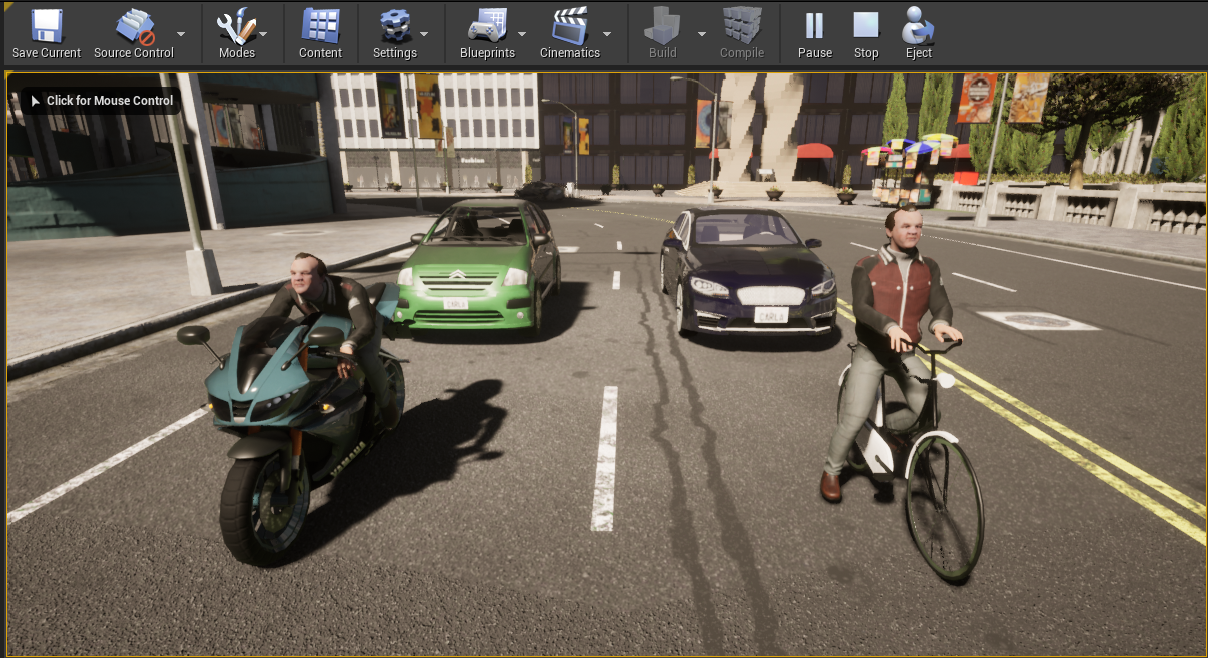
\includegraphics[width=\textwidth]{Figures/biker-cyclist.png}
\caption{CARLA simulator added actors}
\label{fig:biker-cyclist}
\end{figure}


%%%%%%%%%%%%%%%%%%%%%%%%%%%%%%%%%%%%%%%%%%%%%%%%%%%%%%%%%%%%%%%%%%%%%%%%%%%%%
% RUN 003 - Adding dynamic weather
%%%%%%%%%%%%%%%%%%%%%%%%%%%%%%%%%%%%%%%%%%%%%%%%%%%%%%%%%%%%%%%%%%%%%%%%%%%%%
\subsection{Run 003 - Adding dynamic weather}
\label{app_res:003}
\begin{verbatim}
Commit: bb4b95e0
Environment: Local desktop
Command:
$ make launch-only
# In another terminal, change directory to PythonAPI/examples, and run
$ python dynamic_weather.py -s 0.01
Sun(alt: -18.82, azm: 300.53) Storm(clouds=0%, rain=0%, wind=5%)            ^Z
[1]+  Stopped                 python3 dynamic_weather.py -s 0.01

Comment:
The parameter -s (speed) is a denominator in code, see
update_freq = 0.1 / speed_factor
The smaller the number, the less frequent (slower) are the weather updates, 
the greater the number, the more frequent (faster) are the weather updates.
\end{verbatim}

%%%%%%%%%%%%%%%%%%%%%%%%%%%%%%%%%%%%%%%%%%%%%%%%%%%%%%%%%%%%%%%%%%%%%%%%%%%%%
% RUN 004 - Automatic control
%%%%%%%%%%%%%%%%%%%%%%%%%%%%%%%%%%%%%%%%%%%%%%%%%%%%%%%%%%%%%%%%%%%%%%%%%%%%%
\subsection{Run 004 - Automatic control}
\label{app_res:004}
\begin{verbatim}
Commit: bb4b95e0
Environment: Local desktop
Date: 2021.11.21
Command:
$ make launch-only
# Once loaded, press play
# In another terminal, change directory to PythonAPI/examples, and run
$ python automatic_control.py

Comment:
This launches a pygame terminal, with a random vehicle set to ran
\end{verbatim}

%%%%%%%%%%%%%%%%%%%%%%%%%%%%%%%%%%%%%%%%%%%%%%%%%%%%%%%%%%%%%%%%%%%%%%%%%%%%%
% RUN 005 - Automatic control with traffic
%%%%%%%%%%%%%%%%%%%%%%%%%%%%%%%%%%%%%%%%%%%%%%%%%%%%%%%%%%%%%%%%%%%%%%%%%%%%%
\subsection{Run 005 - Automatic control with traffic}
\label{app_res:005}
\begin{verbatim}
Commit: bb4b95e0
Environment: Local desktop
Date: 2021.11.21
Command:
$ make launch-only
# Once loaded, press play
# In another terminal, change directory to PythonAPI/examples, and run
$ python generate_traffic.py 
spawned 30 vehicles and 10 walkers, press Ctrl+C to exit.

# In another terminal, change directory to PythonAPI/examples, and run
$ python automatic_control.py

Comment:
Traffic and automatic control vehicle are visible both in the pygame and unreal 
engine screens.
\end{verbatim}

%%%%%%%%%%%%%%%%%%%%%%%%%%%%%%%%%%%%%%%%%%%%%%%%%%%%%%%%%%%%%%%%%%%%%%%%%%%%%
% RUN 006 - Automatic control with traffic and dynamic weather
%%%%%%%%%%%%%%%%%%%%%%%%%%%%%%%%%%%%%%%%%%%%%%%%%%%%%%%%%%%%%%%%%%%%%%%%%%%%%
\subsection{Run 006- Automatic control with traffic and dynamic weather}
\label{app_res:006}
\begin{verbatim}
Commit: bb4b95e0
Environment: Local desktop
Date: 2021.11.21
Command:
$ make launch-only
# Once loaded, press play
# In another terminal, change directory to PythonAPI/examples, and run
$ python generate_traffic.py 
spawned 30 vehicles and 10 walkers, press Ctrl+C to exit.

# In another terminal, change directory to PythonAPI/examples, and run
$ python dynamic_weather.py -s 0.05
Sun(alt: -19.78, azm: 300.10) Storm(clouds=0%, rain=0%, wind=5%)  

# In another terminal, change directory to PythonAPI/examples, and run
$ python automatic_control.py

Comment:
The sun position changes every two seconds when parameter -s 0.05 is 
passed (0.1 / 0.05 = 2)

To exit the simulation:
1. Ensure dynamic_weather.py is not running or stop with CONTROL + C
2. Stop generate_traffic.py with CONTROL + C
3. Stop dynamic_weather.py with CONTROL + C
4. Stop Unreal Engine

If script generate_traffic.py is not stopped with CONTROL + C, and say CONTROL + Z, may still be running in the background. This will keep a lock on the port.

To list processes (open files) that have port 2000 open:
$ sudo lsof -t -i:2000
3281
3416

To check which process the process ID listed refers to:
$ ps aux | grep 3281
daniel    3281  0.9  0.2 1860476 90348 pts/1   Tl   17:25   0:29 python3 generate_traffic.py
daniel    7455  0.0  0.0  14432  1040 pts/1    S+   18:18   0:00 grep --color=auto 3281

To kill the process:
$ sudo kill -9 3281
[1]+  Killed                  python3 generate_traffic.py

\end{verbatim}

\begin{figure}[h!]
\centering
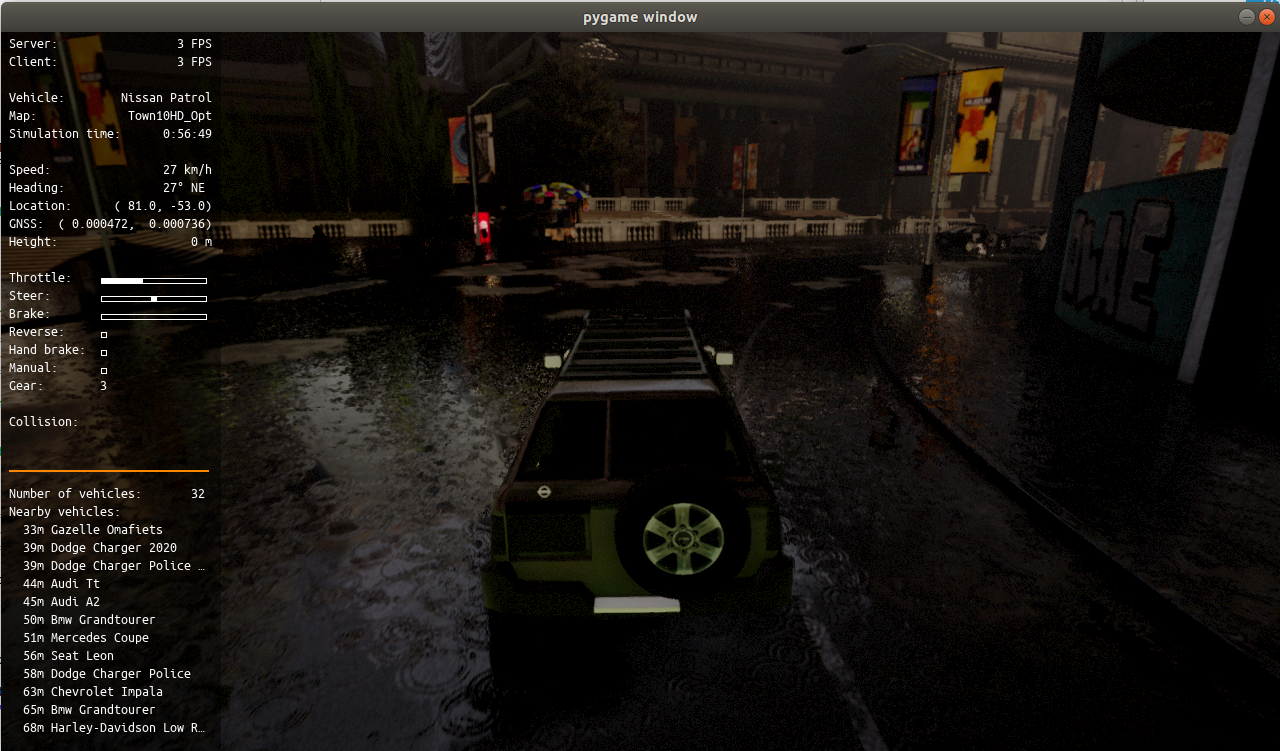
\includegraphics[width=\textwidth]{Figures/carla-rain.png}
\caption{CARLA simulator with dynamic weather}
\label{fig:carla-rain}
\end{figure}

\begin{figure}[h!]
\centering
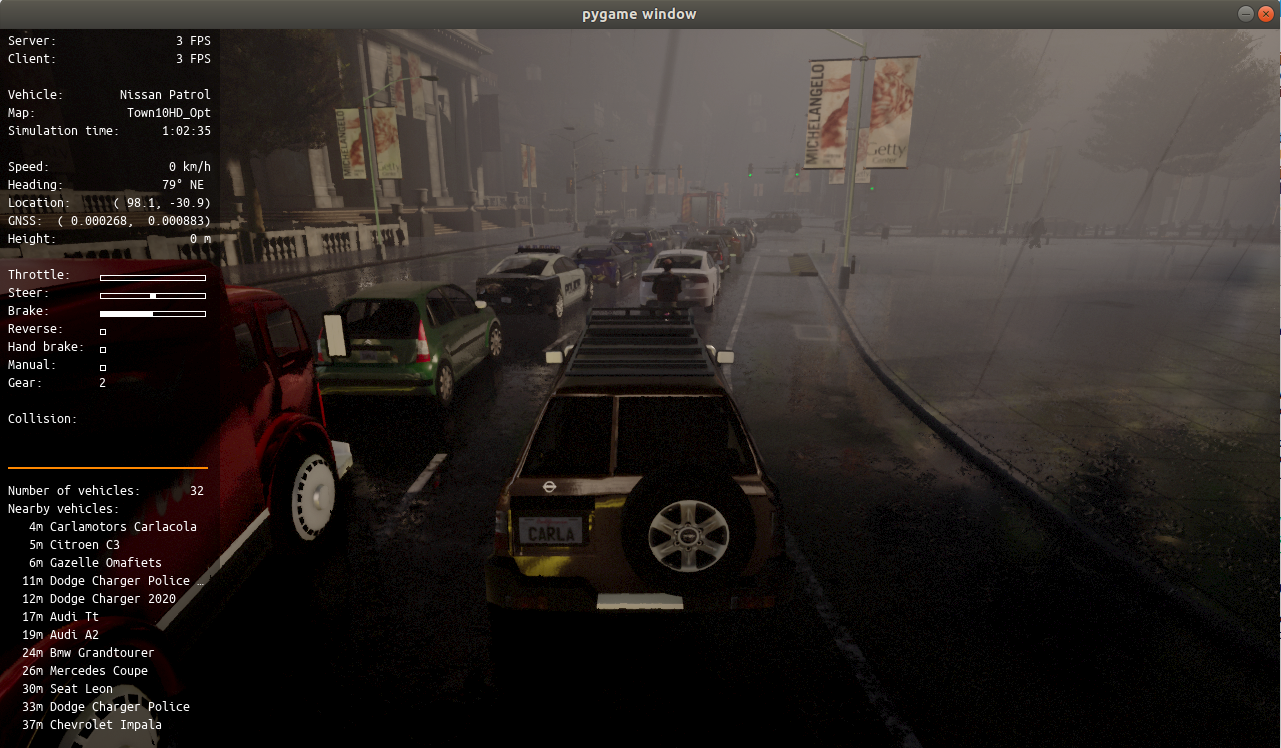
\includegraphics[width=\textwidth]{Figures/carla-traffic-jam.png}
\caption{CARLA simulator traffic jam}
\label{fig:carla-traffic-jam}
\end{figure}

Figures \ref{fig:carla-rain} and \ref{fig:carla-traffic-jam} are taken from the pygame screen.

\begin{figure}[h!]
\centering
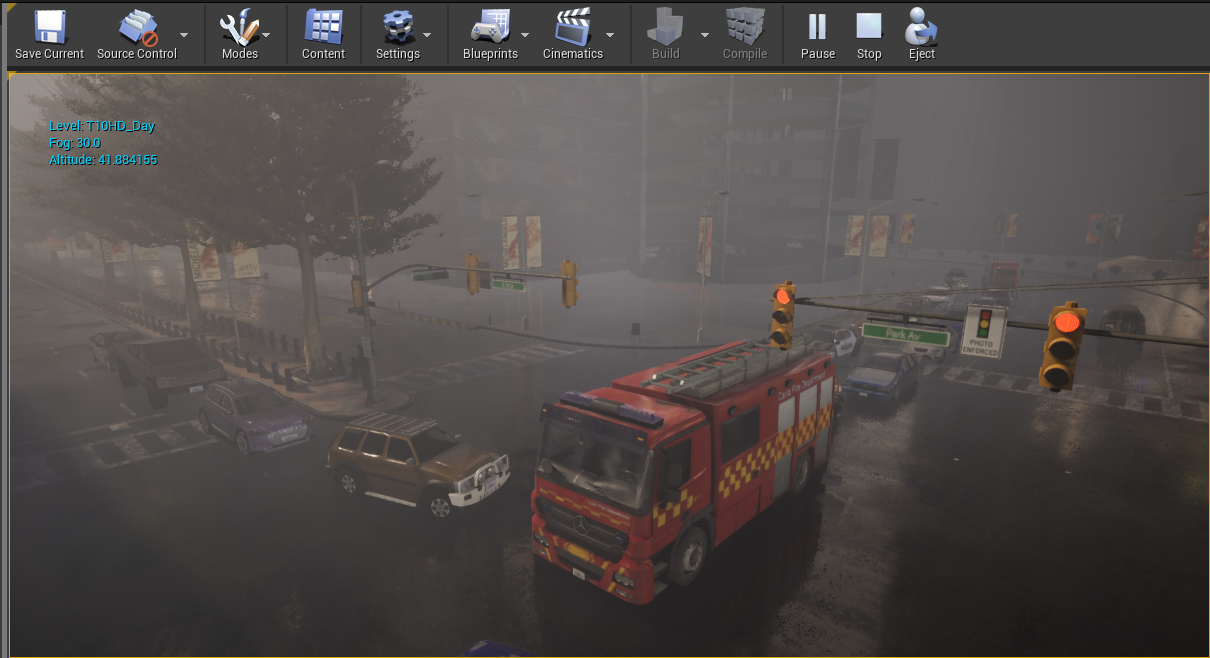
\includegraphics[width=\textwidth]{Figures/carla-traffic-jam-2.png}
\caption{CARLA simulator traffic jam reverse angle}
\label{fig:carla-traffic-jam-2}
\end{figure}

Figure \ref{fig:carla-traffic-jam-2}, taken from Unreal Engine, showing the stopped vehicles at the T-junction and is the reverse angle of Figure \ref{fig:carla-traffic-jam}. note there has not been a collision. The algorithm driving each vehicle seems to be stuck by a proximity assessment that is unlikely to change given all vehicles are stopped.

%%%%%%%%%%%%%%%%%%%%%%%%%%%%%%%%%%%%%%%%%%%%%%%%%%%%%%%%%%%%%%%%%%%%%%%%%%%%%
% RUN 007 - Automatic control with traffic
%%%%%%%%%%%%%%%%%%%%%%%%%%%%%%%%%%%%%%%%%%%%%%%%%%%%%%%%%%%%%%%%%%%%%%%%%%%%%
\subsection{Run 007- Automatic control with traffic}
\label{app_res:007}
\begin{verbatim}
Commit: bb4b95e0
Environment: Local desktop
Date: 2021.11.22
Commands:
$ make launch-only
# Loaded Town04_Opt
$ python generate_traffic.py -n 60 -w 600
spawned 60 vehicles and 328 walkers, press Ctrl+C to exit.
# NB some walkers not created due to collisions
# In another terminal, change directory to PythonAPI/examples, and run
$ python automatic_control.py

Comment:
Various successive runs, number of vehicles decreasing over time due to collisions. One simulated self-drving vehicle got stuck in the simulation (tipycally it would be destroyed at the end of self-driving simulation) after crashing against a traffic-light post.
\end{verbatim}

%%%%%%%%%%%%%%%%%%%%%%%%%%%%%%%%%%%%%%%%%%%%%%%%%%%%%%%%%%%%%%%%%%%%%%%%%%%%%
% RUN 008 - Using the same vehicle
%%%%%%%%%%%%%%%%%%%%%%%%%%%%%%%%%%%%%%%%%%%%%%%%%%%%%%%%%%%%%%%%%%%%%%%%%%%%%
\subsection{Run 008 - Using the same vehicle}
\label{app_res:008}
\begin{verbatim}
Commit: bb4b95e0
Environment: Local desktop
Date: 2021.12.05
Commands:
$ make launch-only
# Loaded Town10HD_Opt (current default)
# pressed "Play"
# generated dynamic weather
$ python dynamic_weather.py --speed 0.1
# generate traffic
$ python generate_traffic.py -n 60 -w 600
(...)
Vehicle agent not added to the crowd by some problem!
(...)
# error message assumed to caused by starting sequence i.e. dynamic weather before dynamic traffic.
$ python generate_traffic.py -n 60 -w 600

Comment:
Currently code uses a random vehicle chosen in automatic_control.py. All cars vanished from simulation two hours in. Pedestrians still present.
\end{verbatim}


%%%%%%%%%%%%%%%%%%%%%%%%%%%%%%%%%%%%%%%%%%%%%%%%%%%%%%%%%%%%%%%%%%%%%%%%%%%%%
% RUN 009 - Hyperion test
%%%%%%%%%%%%%%%%%%%%%%%%%%%%%%%%%%%%%%%%%%%%%%%%%%%%%%%%%%%%%%%%%%%%%%%%%%%%%
\subsection{Run 009 - Hyperion High Computing Cluster Test}
\label{app_res:009}
\begin{verbatim}

% Repository: https://github.com/dsikar/mscai
% Branch: master
% Commit: d4409a20
% Environment: Hyperion
% Date: 2022.03.20
% Connection details:
% As per "HPC - How to connect using windows"
% Commands:
% $ cd ~/localscratch 
% $ git clone https://github.com/dsikar/mscai
% $ cd Lab1
% # deactivate environment - activated by default in ~/.bashrc
% $ flight env deactivate
% # run
% $ source /opt/flight/etc/setup.sh
% $ flight env activate singularity
% $ singularity exec --nv /mnt/scratch/singularity/psarin/ubuntu20_04cuda11.sif   /usr/bin/python3 /users/aczd097/localscratch/mscai/Lab1/DLIALab1.py

% Comment:
% This script is supposed to run with 
% aczd097@login1 ~/localscratch/mscai/Lab1 (master)$ sbatch runModel.sh
% Submitted batch job 173522

% The JOBID does not appear in the queue. Assumption is job fails to start. Also, could be that access to gpu is currently restricted until end of term, as priority is for MScAI students.

% from: https://sylabs.io/guides/3.7/user-guide/definition_files.html
% The process of creating the singularity container (.sif file) is:

% 1. A script is created:
% /mnt/scratch/singularity/psarin/ubuntu20_04cuda11.def
% 2. And built:
% $ sudo singularity build --notest my_container.sif my_container.def

% # Proxy servers
% See: "HPC - Using the proxy server to install software from the internet"
% https://cityuni.service-now.com/sp?id=kb_article_view&sysparm_article=KB0012656

% # HPC - Environment modules
% Search HPC in Service Now

% # online help

% aczd097@login1 ~/fluent $ flight howto list

% | Index | Name                             |

% | 1     | Get Started                      |
% | 2     | Work With The Flight Environment |
% | 3     | Use Flight User Suite            |
% | 4     | Run Jobs                         |
% | 5     | Use A Scheduler                  |
% | 6     | Flight Desktop                   |
% | 7     | Flight Env                       |
% | 8     | Flight Job                       |

% aczd097@login1 ~/fluent $ flight howto show "Get Started"
% HOW TO GET STARTED(7)  Miscellaneous Information Manual  HOW TO GET STARTED(7)
% (...)

% <singularity{+}> [aczd097@login1 [hyperion] git]$ flight help env
%                                    __ _ _       _     _  ==>
%    ==>                            / _| (_)     | |   | |  ==>
%   ==>   ___   _ __    ___  _ __  | |_| |_  __ _| |__ | |_  ==>
%  ==>   / _ \ | '_ \  / _ \| '_ \ |  _| | |/ _` | '_ \| __|  ==>
% ==>   | (_) || |_) ||  __/| | | || | | | | (_| | | | | |_    ==>
%  ==>   \___/ | .__/  \___||_| |_||_| |_|_|\__, |_| |_|\__|  ==>
%   ==>        |_|                           __/ |           ==>
%    ==>  Flight Environment                |___/           ==>
%     ==>  v1.4.0

%   NAME:

%     flight env

%   DESCRIPTION:

%     Manage and access HPC application environments.

%   COMMANDS:

%     activate     Activate an application environment
%     avail        Show available application environment types
%     create       Create a new application environment
%     deactivate   Deactivate the current application environment
%     help         Display global or [command] help documentation
%     info         Show information about an application environment type
%     list         List configured application environments
%     purge        Purge an existing application environment
%     set-default  Set the default application environment
%     show-active  Show currently active application environment
%     show-default Show the default application environment
%     switch       Switch to a different application environment

% <singularity{+}> [aczd097@login1 [hyperion] git]$ flight env avail

% 
% | Name        | Summary                                                                                               |
%
% | brew        | The Missing Package Manager for macOS (or Linux)                                                      |
% |             |                                                                                                       |
% |             |  > https://brew.sh/                                                                                   |
% |             |                                                                                                       |
% | conda       | Package, dependency and environment management for any language.                                      |
% |             |                                                                                                       |
% |             |  > https://conda.io/                                                                                  |
% |             |                                                                                                       |
% | easybuild   | Software build and installation framework.                                                            |
% |             |                                                                                                       |
% |             |  > https://easybuilders.github.io/easybuild/                                                          |
% |             |                                                                                                       |
% | gridware    | Tool for installing and managing scientific applications and libraries.                               |
% |             |                                                                                                       |
% |             |  > https://gridware.alces-flight.com/                                                                 |
% |             |                                                                                                       |
% | modules     | Provides dynamic modification of a user's environment.                                                |
% |             |                                                                                                       |
% |             |  > http://modules.sourceforge.net/                                                                    |
% |             |                                                                                                       |
% | singularity | Container solution for scientific and application driven workloads.                                   |
% |             |                                                                                                       |
% |             |  > https://www.sylabs.io/                                                                             |
% |             |                                                                                                       |
% | spack       | A flexible package manager that supports multiple versions, configurations, platforms, and compilers. |
% |             |  > https://spack.io/                                                                                  |
% |             |                                                                                                       |


\end{verbatim}


%%%%%%%%%%%%%%%%%%%%%%%%%%%%%%%%%%%%%%%%%%%%%%%%%%%%%%%%%%%%%%%%%%%%%%%%%%%%%
% RUN 010 - Dynamic weather
%%%%%%%%%%%%%%%%%%%%%%%%%%%%%%%%%%%%%%%%%%%%%%%%%%%%%%%%%%%%%%%%%%%%%%%%%%%%%
\subsection{Run 010 - Dynamic Weather}
\label{app_res:010}
\begin{verbatim}

Commit: bb4b95e0
Environment: Local desktop
Date: 2021.12.05
Commands:
$ make launch-only
# Loaded Town10HD_Opt (current default)
# pressed "Play"
# generated dynamic weather
$ python dynamic_weather.py --speed 0.1
# generate traffic
$ python generate_traffic.py -n 60 -w 600
(...)
Vehicle agent not added to the crowd by some problem!
(...)
# error message assumed to caused by starting sequence i.e. dynamic weather before dynamic traffic.
$ python generate_traffic.py -n 60 -w 600

Comment:
Currently code uses a random vehicle chosen in automatic_control.py. All cars vanished from simulation two hours in. Pedestrians still present.

\end{verbatim}

%%%%%%%%%%%%%%%%%%%%%%%%%%%%%%%%%%%%%%%%%%%%%%%%%%%%%%%%%%%%%%%%%%%%%%%%%%%%%
% RUN 010 - CIFAR10 Vanilla CNN
%%%%%%%%%%%%%%%%%%%%%%%%%%%%%%%%%%%%%%%%%%%%%%%%%%%%%%%%%%%%%%%%%%%%%%%%%%%%%
\subsection{Run 010 - CIFAR10 Vanilla CNN}
\label{app_res:010}
\begin{verbatim}
Repository: https://github.com/dsikar/quant
Commit: aae016eab3
Environment: Local GPU
Date: 2023.07.23
Commands: python vanilla_cnn_quant.py

\end{verbatim}


%%%%%%%%%%%%%%%%%%%%%%%%%%%%%%%%%%%%%%%%%%%%%%%%%%%%%%%%%%%%%%%%%%%%%%%%%%%%%
% RUN 011 - Contrast test
%%%%%%%%%%%%%%%%%%%%%%%%%%%%%%%%%%%%%%%%%%%%%%%%%%%%%%%%%%%%%%%%%%%%%%%%%%%%%
\subsection{Run 011- Contrast test}
\label{app_res:011}
\begin{verbatim}
Repository: git@github.com:dsikar/ecai2023
Commit: 62fbc1a
Environment: Local GPU
Date: 2023.10.15
Commands: python unit-tests.py
\end{verbatim}

Note, the number of bins used here was 21.

\begin{figure}[h]
\begin{center}
%\framebox[4.0in]{$\;$}
%\fbox{\rule[-.5cm]{0cm}{4cm} \rule[-.5cm]{4cm}{0cm}}
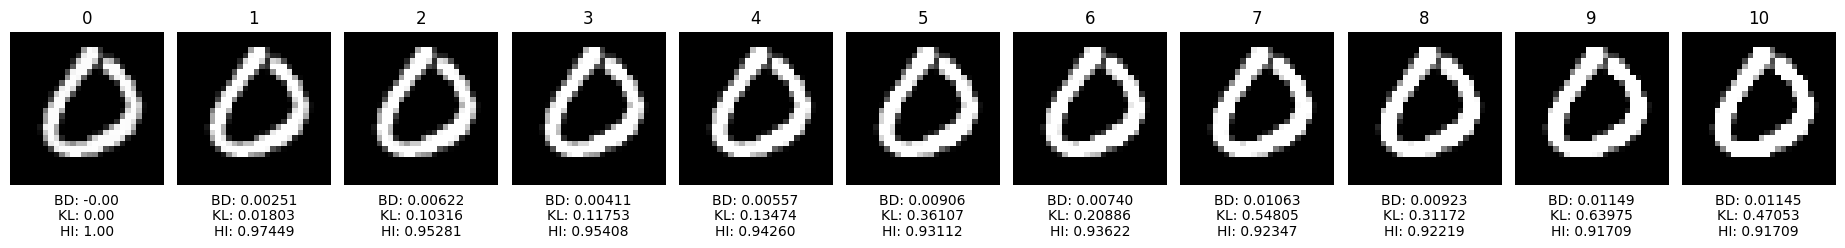
\includegraphics[width=\textwidth]{Figures/Appendixes/brightenss_perturbations_21_bins_27d2880.png}
\end{center}
\caption{Modifying brightness for an MNIST image of the number 0, using 21 bins.}
\end{figure}

%%%%%%%%%%%%%%%%%%%%%%%%%%%%%%%%%%%%%%%%%%%%%%%%%%%%%%%%%%%%%%%%%%%%%%%%%%%%%
% RUN 012 - Contrast test
%%%%%%%%%%%%%%%%%%%%%%%%%%%%%%%%%%%%%%%%%%%%%%%%%%%%%%%%%%%%%%%%%%%%%%%%%%%%%
\subsection{Run 012- Contrast test}
\label{app_res:012}
\begin{verbatim}
Repository: git@github.com:dsikar/ecai2023
Commit: 2c7ca28
Environment: Local GPU
Date: 2023.10.15
Commands: python unit-tests.py
\end{verbatim}

Note, the number of bins used here was 30.

\begin{figure}[h]
\begin{center}
%\framebox[4.0in]{$\;$}
%\fbox{\rule[-.5cm]{0cm}{4cm} \rule[-.5cm]{4cm}{0cm}}
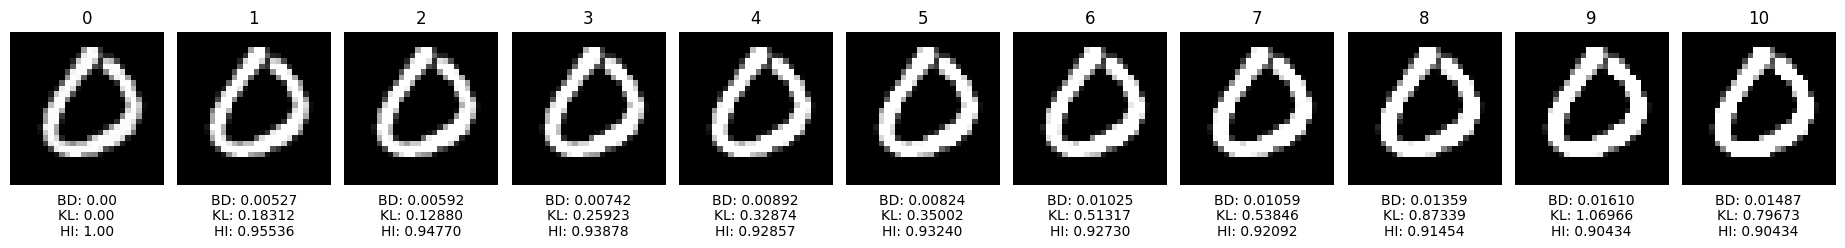
\includegraphics[width=\textwidth]{Figures/Appendixes/brightness_perturbations_30_bins.png}
\end{center}
\caption{Modifying brightness for an MNIST image of the number 0, using 30 bins.}
\end{figure}


%%%%%%%%%%%%%%%%%%%%%%%%%%%%%%%%%%%%%%%%%%%%%%%%%%%%%%%%%%%%%%%%%%%%%%%%%%%%%
% RUN 013 - MNIST Preliminary results
%%%%%%%%%%%%%%%%%%%%%%%%%%%%%%%%%%%%%%%%%%%%%%%%%%%%%%%%%%%%%%%%%%%%%%%%%%%%%
\subsection{Run 013- MNIST preliminary results}
\label{app_res:013}
\begin{verbatim}
Repository: git@github.com:dsikar/ecai2023
Commit: ca91409
Environment: Local GPU
Date: 2023.10.29
Commands: python mnist_cnn_generate_tables.py
\end{verbatim}

Some preliminary data, stored results in scripts/data. Note, need to work on the perturbation levels, to try to match the accuracy to noise levels across all perturbation types.

%%%%%%%%%%%%%%%%%%%%%%%%%%%%%%%%%%%%%%%%%%%%%%%%%%%%%%%%%%%%%%%%%%%%%%%%%%%%%
% RUN 014 - MNIST Preliminary results changed contrast
%%%%%%%%%%%%%%%%%%%%%%%%%%%%%%%%%%%%%%%%%%%%%%%%%%%%%%%%%%%%%%%%%%%%%%%%%%%%%
\subsection{Run 014- MNIST evaluating constrast levels}
\label{app_res:014}
\begin{verbatim}
Repository: git@github.com:dsikar/work-in-progress
Commit: 95be2d0
Environment: Local GPU
Date: 2023.11.19
Commands: python mnist_cnn_eval.py
\end{verbatim}

Modifying the ordering in contrast levels, such that accuracy will decrease as perturbation level increases.

Note, repository name changed from git@github.com:dsikar/ecai2023 to git@github.com:dsikar/work-in-progress.

% Accuracy: 95.8300, with perturbation type contrast values = {'contrast_level': 2.9}, Bhattacharyya Distance: 0.0234, KL Divergence: 1.7614, Histogram Intersection: 0.9053
% Accuracy: 95.5800, with perturbation type contrast values = {'contrast_level': 2.8}, Bhattacharyya Distance: 0.0233, KL Divergence: 1.7473, Histogram Intersection: 0.9056
% Accuracy: 95.1400, with perturbation type contrast values = {'contrast_level': 2.7}, Bhattacharyya Distance: 0.0232, KL Divergence: 1.7322, Histogram Intersection: 0.9058
% Accuracy: 94.8900, with perturbation type contrast values = {'contrast_level': 2.6}, Bhattacharyya Distance: 0.0231, KL Divergence: 1.7221, Histogram Intersection: 0.9061
% Accuracy: 94.4500, with perturbation type contrast values = {'contrast_level': 2.5}, Bhattacharyya Distance: 0.0230, KL Divergence: 1.7080, Histogram Intersection: 0.9063
% Accuracy: 94.0300, with perturbation type contrast values = {'contrast_level': 2.4}, Bhattacharyya Distance: 0.0229, KL Divergence: 1.6932, Histogram Intersection: 0.9066
% Accuracy: 93.5400, with perturbation type contrast values = {'contrast_level': 2.3}, Bhattacharyya Distance: 0.0228, KL Divergence: 1.6782, Histogram Intersection: 0.9070
% Accuracy: 93.0300, with perturbation type contrast values = {'contrast_level': 2.2}, Bhattacharyya Distance: 0.0226, KL Divergence: 1.6614, Histogram Intersection: 0.9073
% Accuracy: 92.4100, with perturbation type contrast values = {'contrast_level': 2.1}, Bhattacharyya Distance: 0.0225, KL Divergence: 1.6498, Histogram Intersection: 0.9075
% Accuracy: 91.7900, with perturbation type contrast values = {'contrast_level': 2.0}, Bhattacharyya Distance: 0.0224, KL Divergence: 1.6375, Histogram Intersection: 0.9078
% Accuracy: 91.0100, with perturbation type contrast values = {'contrast_level': 1.9}, Bhattacharyya Distance: 0.0223, KL Divergence: 1.6164, Histogram Intersection: 0.9082
% Accuracy: 90.2900, with perturbation type contrast values = {'contrast_level': 1.8}, Bhattacharyya Distance: 0.0221, KL Divergence: 1.6051, Histogram Intersection: 0.9086
% Accuracy: 89.4800, with perturbation type contrast values = {'contrast_level': 1.7}, Bhattacharyya Distance: 0.0219, KL Divergence: 1.5845, Histogram Intersection: 0.9090
% Accuracy: 88.7600, with perturbation type contrast values = {'contrast_level': 1.6}, Bhattacharyya Distance: 0.0218, KL Divergence: 1.5692, Histogram Intersection: 0.9094
% Accuracy: 87.8000, with perturbation type contrast values = {'contrast_level': 1.5}, Bhattacharyya Distance: 0.0217, KL Divergence: 1.5511, Histogram Intersection: 0.9098
% Accuracy: 87.0500, with perturbation type contrast values = {'contrast_level': 1.4}, Bhattacharyya Distance: 0.0215, KL Divergence: 1.5365, Histogram Intersection: 0.9102
% Accuracy: 86.5100, with perturbation type contrast values = {'contrast_level': 1.3}, Bhattacharyya Distance: 0.0214, KL Divergence: 1.5199, Histogram Intersection: 0.9107
% Accuracy: 85.9600, with perturbation type contrast values = {'contrast_level': 1.2}, Bhattacharyya Distance: 0.0212, KL Divergence: 1.4996, Histogram Intersection: 0.9113
% Accuracy: 85.4700, with perturbation type contrast values = {'contrast_level': 1.1}, Bhattacharyya Distance: 0.0210, KL Divergence: 1.4771, Histogram Intersection: 0.9119
% Accuracy: 85.0700, with perturbation type contrast values = {'contrast_level': 1.0}, Bhattacharyya Distance: 0.0208, KL Divergence: 1.4600, Histogram Intersection: 0.9125
% Accuracy: 84.3400, with perturbation type contrast values = {'contrast_level': 0.9}, Bhattacharyya Distance: 0.0207, KL Divergence: 1.4402, Histogram Intersection: 0.9131
% Accuracy: 83.9800, with perturbation type contrast values = {'contrast_level': 0.8}, Bhattacharyya Distance: 0.0205, KL Divergence: 1.4202, Histogram Intersection: 0.9139
% Accuracy: 83.5500, with perturbation type contrast values = {'contrast_level': 0.7}, Bhattacharyya Distance: 0.0203, KL Divergence: 1.3963, Histogram Intersection: 0.9147
% Accuracy: 83.0200, with perturbation type contrast values = {'contrast_level': 0.6}, Bhattacharyya Distance: 0.0200, KL Divergence: 1.3659, Histogram Intersection: 0.9157
% Accuracy: 82.4400, with perturbation type contrast values = {'contrast_level': 0.5}, Bhattacharyya Distance: 0.0197, KL Divergence: 1.3381, Histogram Intersection: 0.9167
% Accuracy: 81.8100, with perturbation type contrast values = {'contrast_level': 0.4}, Bhattacharyya Distance: 0.0195, KL Divergence: 1.3016, Histogram Intersection: 0.9178
% Accuracy: 81.0200, with perturbation type contrast values = {'contrast_level': 0.3}, Bhattacharyya Distance: 0.0192, KL Divergence: 1.2624, Histogram Intersection: 0.9191
% Accuracy: 80.0600, with perturbation type contrast values = {'contrast_level': 0.2}, Bhattacharyya Distance: 0.0188, KL Divergence: 1.2234, Histogram Intersection: 0.9206
% Accuracy: 79.1800, with perturbation type contrast values = {'contrast_level': 0.1}, Bhattacharyya Distance: 0.0184, KL Divergence: 1.1720, Histogram Intersection: 0.9224
% Accuracy: 84.3400, with perturbation type contrast values = {'contrast_level': 0.9}, Bhattacharyya Distance: 0.0207, KL Divergence: 1.4402, Histogram Intersection: 0.9131
% Accuracy: 83.9800, with perturbation type contrast values = {'contrast_level': 0.8}, Bhattacharyya Distance: 0.0205, KL Divergence: 1.4202, Histogram Intersection: 0.9139
% Accuracy: 83.5500, with perturbation type contrast values = {'contrast_level': 0.7}, Bhattacharyya Distance: 0.0203, KL Divergence: 1.3963, Histogram Intersection: 0.9147
% Accuracy: 83.0200, with perturbation type contrast values = {'contrast_level': 0.6}, Bhattacharyya Distance: 0.0200, KL Divergence: 1.3659, Histogram Intersection: 0.9157
% Accuracy: 82.4400, with perturbation type contrast values = {'contrast_level': 0.5}, Bhattacharyya Distance: 0.0197, KL Divergence: 1.3381, Histogram Intersection: 0.9167
% Accuracy: 81.8100, with perturbation type contrast values = {'contrast_level': 0.4}, Bhattacharyya Distance: 0.0195, KL Divergence: 1.3016, Histogram Intersection: 0.9178
% Accuracy: 81.0200, with perturbation type contrast values = {'contrast_level': 0.3}, Bhattacharyya Distance: 0.0192, KL Divergence: 1.2624, Histogram Intersection: 0.9191
% Accuracy: 80.0600, with perturbation type contrast values = {'contrast_level': 0.2}, Bhattacharyya Distance: 0.0188, KL Divergence: 1.2234, Histogram Intersection: 0.9206
% Accuracy: 79.1800, with perturbation type contrast values = {'contrast_level': 0.1}, Bhattacharyya Distance: 0.0184, KL Divergence: 1.1720, Histogram Intersection: 0.9224
% Accuracy: 78.3400, with perturbation type contrast values = {'contrast_level': 0.0}, Bhattacharyya Distance: 0.0179, KL Divergence: 1.1160, Histogram Intersection: 0.9247
% Accuracy: 77.0800, with perturbation type contrast values = {'contrast_level': -0.1}, Bhattacharyya Distance: 0.0174, KL Divergence: 1.0530, Histogram Intersection: 0.9272
% Accuracy: 75.2700, with perturbation type contrast values = {'contrast_level': -0.2}, Bhattacharyya Distance: 0.0169, KL Divergence: 0.9794, Histogram Intersection: 0.9306
% Accuracy: 73.4300, with perturbation type contrast values = {'contrast_level': -0.3}, Bhattacharyya Distance: 0.0158, KL Divergence: 0.8528, Histogram Intersection: 0.9369
% Accuracy: 70.9200, with perturbation type contrast values = {'contrast_level': -0.4}, Bhattacharyya Distance: 0.0089, KL Divergence: 0.4424, Histogram Intersection: 0.9652
% Accuracy: 65.2400, with perturbation type contrast values = {'contrast_level': -0.5}, Bhattacharyya Distance: 0.0001, KL Divergence: 0.0018, Histogram Intersection: 0.9997
% Accuracy: 54.8700, with perturbation type contrast values = {'contrast_level': -0.6}, Bhattacharyya Distance: 0.0001, KL Divergence: 0.0039, Histogram Intersection: 0.9994
% Accuracy: 38.7700, with perturbation type contrast values = {'contrast_level': -0.7}, Bhattacharyya Distance: 0.0001, KL Divergence: 0.0031, Histogram Intersection: 0.9995
% Accuracy: 16.6700, with perturbation type contrast values = {'contrast_level': -0.8}, Bhattacharyya Distance: 0.0001, KL Divergence: 0.0025, Histogram Intersection: 0.9995
% Accuracy: 9.7400, with perturbation type contrast values = {'contrast_level': -0.9}, Bhattacharyya Distance: 0.0001, KL Divergence: 0.0030, Histogram Intersection: 0.9994
% Accuracy: 9.7400, with perturbation type contrast values = {'contrast_level': -1.0}, Bhattacharyya Distance: -1.3617, KL Divergence: 28.6177, Histogram Intersection: 0.0033

%%%%%%%%%%%%%%%%%%%%%%%%%%%%%%%%%%%%%%%%%%%%%%%%%%%%%%%%%%%%%%%%%%%%%%%%%%%%%
% RUN 015 - MNIST Contrast Levels
%%%%%%%%%%%%%%%%%%%%%%%%%%%%%%%%%%%%%%%%%%%%%%%%%%%%%%%%%%%%%%%%%%%%%%%%%%%%%
\subsection{Run 015 - MNIST contrast level plots}
\label{app_res:015}
\begin{verbatim}
Repository: git@github.com:dsikar/work-in-progress
Commit: 5399d69
Environment: Local GPU
Date: 2023.11.26
Commands: python contrast_levels.py
\end{verbatim}

\begin{table}[ht]
\centering
\begin{tabular}{|c|c|c|c|c|}
\hline
Contrast Level & Accuracy & BD & KL & HI \\
\hline
3.0 & 96.0000 & 0.0235 & 1.7749 & 0.9050 \\
2.9 & 95.8300 & 0.0234 & 1.7614 & 0.9053 \\
2.8 & 95.5800 & 0.0233 & 1.7473 & 0.9056 \\
2.7 & 95.1400 & 0.0232 & 1.7322 & 0.9058 \\
2.6 & 94.8900 & 0.0231 & 1.7221 & 0.9061 \\
2.5 & 94.4500 & 0.0230 & 1.7080 & 0.9063 \\
2.4 & 94.0300 & 0.0229 & 1.6932 & 0.9066 \\
2.3 & 93.5400 & 0.0228 & 1.6782 & 0.9070 \\
2.2 & 93.0300 & 0.0226 & 1.6614 & 0.9073 \\
2.1 & 92.4100 & 0.0225 & 1.6498 & 0.9075 \\
2.0 & 91.7900 & 0.0224 & 1.6375 & 0.9078 \\
1.9 & 91.0100 & 0.0223 & 1.6164 & 0.9082 \\
1.8 & 90.2900 & 0.0221 & 1.6051 & 0.9086 \\
1.7 & 89.4800 & 0.0219 & 1.5845 & 0.9090 \\
1.6 & 88.7600 & 0.0218 & 1.5692 & 0.9094 \\
1.5 & 87.8000 & 0.0217 & 1.5511 & 0.9098 \\
1.4 & 87.0500 & 0.0215 & 1.5365 & 0.9102 \\
1.3 & 86.5100 & 0.0214 & 1.5199 & 0.9107 \\
1.2 & 85.9600 & 0.0212 & 1.4996 & 0.9113 \\
1.1 & 85.4700 & 0.0210 & 1.4771 & 0.9119 \\
1.0 & 85.0700 & 0.0208 & 1.4600 & 0.9125 \\
0.9 & 84.3400 & 0.0207 & 1.4402 & 0.9131 \\
0.8 & 83.9800 & 0.0205 & 1.4202 & 0.9139 \\
0.7 & 83.5500 & 0.0203 & 1.3963 & 0.9147 \\
0.6 & 83.0200 & 0.0200 & 1.3659 & 0.9157 \\
0.5 & 82.4400 & 0.0197 & 1.3381 & 0.9167 \\
0.4 & 81.8100 & 0.0195 & 1.3016 & 0.9178 \\
0.3 & 81.0200 & 0.0192 & 1.2624 & 0.9191 \\
0.2 & 80.0600 & 0.0188 & 1.2234 & 0.9206 \\
0.0 & 78.3400 & 0.0179 & 1.1160 & 0.9247 \\
-0.1 & 77.0800 & 0.0174 & 1.0530 & 0.9272 \\
-0.2 & 75.2700 & 0.0169 & 0.9794 & 0.9306 \\
-0.3 & 73.4300 & 0.0158 & 0.8528 & 0.9369 \\
-0.4 & 70.9200 & 0.0089 & 0.4424 & 0.9652 \\
-0.5 & 65.2400 & 0.0001 & 0.0018 & 0.9997 \\
-0.6 & 54.8700 & 0.0001 & 0.0039 & 0.9994 \\
-0.7 & 38.7700 & 0.0001 & 0.0031 & 0.9995 \\
-0.8 & 16.6700 & 0.0001 & 0.0025 & 0.9995 \\
-0.9 & 9.7400 & 0.0001 & 0.0030 & 0.9994 \\
-1.0 & 9.7400 & -1.3617 & 28.6177 & 0.0033 \\

\hline
\end{tabular}
\caption{Experimental contrast levels and resulting Accuracy, Bhatacharya Distance (BD), KL Divergence (KL) and Histogram Intersection (HI) for contrast applied to MNIST testing dataset and resulting accuracy and distance metrics, where accuracy on original testing MNIST Dataset is 98.38\%}
\label{your-label-here}
\end{table}

%%%%%%%%%%%%%%%%%%%%%%%%%%%%%%%%%%%%%%%%%%%%%%%%%%%%%%%%%%%%%%%%%%%%%%%%%%%%%
% RUN 016 - MNIST Brightness Levels
%%%%%%%%%%%%%%%%%%%%%%%%%%%%%%%%%%%%%%%%%%%%%%%%%%%%%%%%%%%%%%%%%%%%%%%%%%%%%
\subsection{Run 016 - MNIST brightness level plot and table}
\label{app_res:016}
\begin{verbatim}
Repository: git@github.com:dsikar/work-in-progress
Commit: 20d96b36
Environment: Local GPU
Date: 2023.12.16
Commands: python contrast_levels.py # edited for brightness
\end{verbatim}

%%%%%%%%%%%%%%%%%%%%%%%%%%%%%%%%%%%%%%%%%%%%%%%%%%%%%%%%%%%%%%%%%%%%%%%%%%%%%
% RUN 017 - MNIST Defocus Blur Levels
%%%%%%%%%%%%%%%%%%%%%%%%%%%%%%%%%%%%%%%%%%%%%%%%%%%%%%%%%%%%%%%%%%%%%%%%%%%%%
\subsection{Run 017 - MNIST defocus level plot and table}
\label{app_res:017}
\begin{verbatim}
Repository: git@github.com:dsikar/work-in-progress
Commit: ee06742
Environment: Local GPU
Date: 2023.12.16
Commands: python mnist_cnn_eval.py 
\end{verbatim}

Results commented out in latex. 

% Accuracy on test dataset: 98.38%
% Perturbation type: defocus_blur
% Accuracy: 98.4000, with perturbation type defocus_blur values = {'kernel_size': 3, 'blur_amount': 0.1}, Bhattacharyya Distance: 0.0168, KL Divergence: 0.3240, Histogram Intersection: 0.9051
% Accuracy: 98.3100, with perturbation type defocus_blur values = {'kernel_size': 3, 'blur_amount': 0.2}, Bhattacharyya Distance: 0.0282, KL Divergence: 0.4355, Histogram Intersection: 0.8472
% Accuracy: 98.2300, with perturbation type defocus_blur values = {'kernel_size': 3, 'blur_amount': 0.3}, Bhattacharyya Distance: 0.0316, KL Divergence: 0.4353, Histogram Intersection: 0.8291
% Accuracy: 98.0300, with perturbation type defocus_blur values = {'kernel_size': 3, 'blur_amount': 0.4}, Bhattacharyya Distance: 0.0334, KL Divergence: 0.4271, Histogram Intersection: 0.8201
% Accuracy: 97.9900, with perturbation type defocus_blur values = {'kernel_size': 3, 'blur_amount': 0.5}, Bhattacharyya Distance: 0.0342, KL Divergence: 0.4022, Histogram Intersection: 0.8156
% Accuracy: 97.7700, with perturbation type defocus_blur values = {'kernel_size': 3, 'blur_amount': 0.6}, Bhattacharyya Distance: 0.0348, KL Divergence: 0.3769, Histogram Intersection: 0.8125
% Accuracy: 97.4800, with perturbation type defocus_blur values = {'kernel_size': 3, 'blur_amount': 0.7}, Bhattacharyya Distance: 0.0354, KL Divergence: 0.3671, Histogram Intersection: 0.8101
% Accuracy: 97.1500, with perturbation type defocus_blur values = {'kernel_size': 3, 'blur_amount': 0.8}, Bhattacharyya Distance: 0.0365, KL Divergence: 0.3710, Histogram Intersection: 0.8069
% Accuracy: 96.7400, with perturbation type defocus_blur values = {'kernel_size': 3, 'blur_amount': 0.9}, Bhattacharyya Distance: 0.0371, KL Divergence: 0.3773, Histogram Intersection: 0.8049
% Accuracy: 96.1100, with perturbation type defocus_blur values = {'kernel_size': 3, 'blur_amount': 1.0}, Bhattacharyya Distance: 0.0377, KL Divergence: 0.3916, Histogram Intersection: 0.8028
% Accuracy: 83.1900, with perturbation type defocus_blur values = {'kernel_size': 5, 'blur_amount': 1.1}, Bhattacharyya Distance: 0.0633, KL Divergence: 0.6136, Histogram Intersection: 0.6863
% Accuracy: 83.4100, with perturbation type defocus_blur values = {'kernel_size': 5, 'blur_amount': 1.2}, Bhattacharyya Distance: 0.0653, KL Divergence: 0.6819, Histogram Intersection: 0.6823
% Accuracy: 84.9200, with perturbation type defocus_blur values = {'kernel_size': 5, 'blur_amount': 1.3}, Bhattacharyya Distance: 0.0670, KL Divergence: 0.7545, Histogram Intersection: 0.6790
% Accuracy: 87.2600, with perturbation type defocus_blur values = {'kernel_size': 5, 'blur_amount': 1.4}, Bhattacharyya Distance: 0.0679, KL Divergence: 0.8066, Histogram Intersection: 0.6774
% Accuracy: 89.2900, with perturbation type defocus_blur values = {'kernel_size': 5, 'blur_amount': 1.5}, Bhattacharyya Distance: 0.0681, KL Divergence: 0.8386, Histogram Intersection: 0.6776
% Accuracy: 90.8200, with perturbation type defocus_blur values = {'kernel_size': 5, 'blur_amount': 1.6}, Bhattacharyya Distance: 0.0675, KL Divergence: 0.8443, Histogram Intersection: 0.6801
% Accuracy: 91.5500, with perturbation type defocus_blur values = {'kernel_size': 5, 'blur_amount': 1.7}, Bhattacharyya Distance: 0.0660, KL Divergence: 0.8252, Histogram Intersection: 0.6847
% Accuracy: 91.4300, with perturbation type defocus_blur values = {'kernel_size': 5, 'blur_amount': 1.8}, Bhattacharyya Distance: 0.0638, KL Divergence: 0.7882, Histogram Intersection: 0.6910
% Accuracy: 90.8100, with perturbation type defocus_blur values = {'kernel_size': 5, 'blur_amount': 1.9}, Bhattacharyya Distance: 0.0611, KL Divergence: 0.7381, Histogram Intersection: 0.6989
% Accuracy: 89.9400, with perturbation type defocus_blur values = {'kernel_size': 5, 'blur_amount': 2.0}, Bhattacharyya Distance: 0.0586, KL Divergence: 0.6823, Histogram Intersection: 0.7065
% Saved to file: vanilla_cnn_mnist_20231217172454.pkl



%%%%%%%%%%%%%%%%%%%%%%%%%%%%%%%%%%%%%%%%%%%%%%%%%%%%%%%%%%%%%%%%%%%%%%%%%%%%%
% RUN 018 - MNIST Fog Levels
%%%%%%%%%%%%%%%%%%%%%%%%%%%%%%%%%%%%%%%%%%%%%%%%%%%%%%%%%%%%%%%%%%%%%%%%%%%%%
\subsection{Run 018 - MNIST fog plot and table}
\label{app_res:018}
\begin{verbatim}
Repository: git@github.com:dsikar/work-in-progress
Commit: e1bea3c
Environment: Local GPU
Date: 2023.12.16
Commands: python mnist_cnn_eval.py 
\end{verbatim}

Added fog levels to work-in-progress.

%%%%%%%%%%%%%%%%%%%%%%%%%%%%%%%%%%%%%%%%%%%%%%%%%%%%%%%%%%%%%%%%%%%%%%%%%%%%%
% RUN 019 - MNIST Gaussian Noise Levels
%%%%%%%%%%%%%%%%%%%%%%%%%%%%%%%%%%%%%%%%%%%%%%%%%%%%%%%%%%%%%%%%%%%%%%%%%%%%%
\subsection{Run 019 - MNIST Gaussian Noise plot and table}
\label{app_res:019}
\begin{verbatim}
Repository: git@github.com:dsikar/work-in-progress
Commit: 0673368
Environment: Local GPU
Date: 2023.12.23
Commands: python gaussian_noise_levels.py 
\end{verbatim}

Added Gaussian levels to work-in-progress.

\begin{table}[ht]
\centering
\begin{tabular}{|c|c|c|c|c|}
\hline
Gaussian Noise Level & Accuracy & BD & KL & HI \\
\hline
1.00 & 98.3300 & 0.0948 & 0.7330 & 0.5408 \\
2.00 & 93.5300 & 0.3278 & 2.5286 & 0.2032 \\
3.00 & 85.9200 & 0.3922 & 3.2614 & 0.1798 \\
4.00 & 80.4900 & 0.4215 & 3.6819 & 0.1733 \\
5.00 & 76.1400 & 0.4476 & 4.1378 & 0.1685 \\
6.00 & 71.5200 & 0.4676 & 4.5594 & 0.1652 \\
7.00 & 66.7400 & 0.4797 & 4.8580 & 0.1632 \\
8.00 & 60.5600 & 0.4849 & 5.0233 & 0.1621 \\
9.00 & 56.0000 & 0.4862 & 5.0806 & 0.1618 \\
10.00 & 50.5300 & 0.4863 & 5.1120 & 0.1616 \\
\hline
\end{tabular}
\caption{Experimental Gaussian noise levels and resulting Accuracy, Bhattacharya Distance (BD), KL Divergence (KL) and Histogram Intersection (HI) for noise applied to MNIST testing dataset and resulting accuracy and distance metrics, where accuracy on original testing MNIST Dataset is 98.38\%}
\label{tbl-fog-levels}
\end{table}

%%%%%%%%%%%%%%%%%%%%%%%%%%%%%%%%%%%%%%%%%%%%%%%%%%%%%%%%%%%%%%%%%%%%%%%%%%%%%
% RUN 020 - MNIST Impulse Noise Levels
%%%%%%%%%%%%%%%%%%%%%%%%%%%%%%%%%%%%%%%%%%%%%%%%%%%%%%%%%%%%%%%%%%%%%%%%%%%%%
\subsection{Run 020 - MNIST Impulse Noise plot and table}
\label{app_res:020}
\begin{verbatim}
Repository: git@github.com:dsikar/work-in-progress
Commit: c755432
Environment: Local GPU
Date: 2023.12.23
Commands:python noise_levels.py "impulse_noise" "Impulse Noise" \
"vanilla_cnn_mnist_20231223171844_impulse_noise.pkl"
\end{verbatim}

\begin{table}[ht]
\centering
\begin{tabular}{|c|c|c|c|c|}
\hline
Gaussian Noise Level & Accuracy & BD & KL & HI \\
\hline
1.00 & 94.8600 & 0.0448 & 0.3418 & 0.7733 \\
2.00 & 88.1200 & 0.0684 & 0.5230 & 0.6844 \\
3.00 & 82.1100 & 0.0817 & 0.6260 & 0.6400 \\
4.00 & 76.9000 & 0.0961 & 0.7402 & 0.5956 \\
5.00 & 71.7200 & 0.1122 & 0.8708 & 0.5501 \\
6.00 & 67.4400 & 0.1295 & 1.0114 & 0.5059 \\
7.00 & 62.9400 & 0.1487 & 1.1693 & 0.4616 \\
8.00 & 58.2700 & 0.1702 & 1.3549 & 0.4175 \\
9.00 & 53.9600 & 0.1948 & 1.5666 & 0.3732 \\
10.00 & 49.8400 & 0.2239 & 1.8144 & 0.3280 \\
\hline
\end{tabular}
\caption{Experimental Impulse noise levels and resulting Accuracy, Bhattacharya Distance (BD), KL Divergence (KL) and Histogram Intersection (HI) for noise applied to MNIST testing dataset and resulting accuracy and distance metrics, where accuracy on original testing MNIST Dataset is 98.38\%}
\label{tbl-impulse-noise-levels}
\end{table}

%%%%%%%%%%%%%%%%%%%%%%%%%%%%%%%%%%%%%%%%%%%%%%%%%%%%%%%%%%%%%%%%%%%%%%%%%%%%%
% RUN 021 - MNIST Motion Blur Levels
%%%%%%%%%%%%%%%%%%%%%%%%%%%%%%%%%%%%%%%%%%%%%%%%%%%%%%%%%%%%%%%%%%%%%%%%%%%%%
\subsection{Run 021 - MNIST Motion plot and table}
\label{app_res:021}
\begin{verbatim}
Repository: git@github.com:dsikar/work-in-progress
Commit: b7af99b
Environment: Local GPU
Date: 2023.12.25
Commands: python3 noise_levels.py motion_blur 'Motion Blur' \
vanilla_cnn_mnist_20231225150838_motion_blur.pkl
\end{verbatim}

\begin{table}[ht]
\centering
\begin{tabular}{|c|c|c|c|c|}
\hline
Motion Blur Level & Accuracy & BD & KL & HI \\
\hline
1.00 & 98.3800 & -0.0000 & 0.0000 & 1.0000 \\
2.00 & 96.1600 & 0.0147 & 0.2763 & 0.9146 \\
3.00 & 96.8900 & 0.0211 & 0.2579 & 0.8752 \\
4.00 & 89.2300 & 0.0284 & 0.3199 & 0.8401 \\
5.00 & 88.3100 & 0.0357 & 0.4014 & 0.8086 \\
6.00 & 73.8400 & 0.0424 & 0.4840 & 0.7809 \\
7.00 & 72.0800 & 0.0490 & 0.5553 & 0.7555 \\
8.00 & 58.1600 & 0.0546 & 0.6127 & 0.7330 \\
9.00 & 56.9600 & 0.0598 & 0.6624 & 0.7131 \\
10.00 & 48.6400 & 0.0642 & 0.6988 & 0.6954 \\
\hline
\end{tabular}
\caption{Experimental Motion Blur levels and resulting Accuracy, Bhattacharya Distance (BD), KL Divergence (KL) and Histogram Intersection (HI) for noise applied to MNIST testing dataset and resulting accuracy and distance metrics, where accuracy on original testing MNIST Dataset is 98.38\%}
\label{tbl-impulse-noise-levels}
\end{table}

%%%%%%%%%%%%%%%%%%%%%%%%%%%%%%%%%%%%%%%%%%%%%%%%%%%%%%%%%%%%%%%%%%%%%%%%%%%%%
% RUN 022 - MNIST Pixelation Levels
%%%%%%%%%%%%%%%%%%%%%%%%%%%%%%%%%%%%%%%%%%%%%%%%%%%%%%%%%%%%%%%%%%%%%%%%%%%%%
\subsection{Run 022 - MNIST Pixelation plot and table}
\label{app_res:022}
\begin{verbatim}
Repository: git@github.com:dsikar/work-in-progress
Commit: 9d09f4a
Environment: Local GPU
Date: 2023.12.25
Commands: python3 noise_levels.py
\end{verbatim}

\begin{table}[ht]
\centering
\begin{tabular}{|c|c|c|c|c|}
\hline
Pixelation Level & Accuracy & BD & KL & HI \\
\hline
1.00 & 97.1500 & 0.0194 & 0.2853 & 0.8876 \\
2.00 & 98.0900 & 0.0332 & 1.1829 & 0.8486 \\
3.00 & 95.0000 & 0.0514 & 1.5079 & 0.7727 \\
4.00 & 93.8400 & 0.0591 & 1.7781 & 0.7436 \\
5.00 & 89.7600 & 0.0665 & 1.9705 & 0.7162 \\
6.00 & 84.0100 & 0.0709 & 2.1510 & 0.7052 \\
7.00 & 84.0100 & 0.0709 & 2.1510 & 0.7052 \\
8.00 & 72.8000 & 0.0882 & 2.3196 & 0.6373 \\
9.00 & 55.5000 & 0.1050 & 2.5272 & 0.5891 \\
10.00 & 43.2100 & 0.1286 & 2.7817 & 0.5322 \\
\hline
\end{tabular}
\caption{Experimental Pixelation levels and resulting Accuracy, Bhattacharya Distance (BD), KL Divergence (KL) and Histogram Intersection (HI) for noise applied to MNIST testing dataset and resulting accuracy and distance metrics, where accuracy on original testing MNIST Dataset is 98.38\%}
\label{tbl-pixelation-levels}
\end{table}

%%%%%%%%%%%%%%%%%%%%%%%%%%%%%%%%%%%%%%%%%%%%%%%%%%%%%%%%%%%%%%%%%%%%%%%%%%%%%
% RUN 023 - MNIST Shot Noise Levels
%%%%%%%%%%%%%%%%%%%%%%%%%%%%%%%%%%%%%%%%%%%%%%%%%%%%%%%%%%%%%%%%%%%%%%%%%%%%%
\subsection{Run 023 - MNIST Shot Noise plot and table}
\label{app_res:023}
\begin{verbatim}
Repository: git@github.com:dsikar/work-in-progress
Commit: 6e3adc0
Environment: Local GPU
Date: 2023.12.25
Commands: python3 noise_levels.py
\end{verbatim}

\begin{table}[ht]
\centering
\begin{tabular}{|c|c|c|c|c|}
\hline
Pixelation Level & Accuracy & BD & KL & HI \\
\hline

1.00 & 97.7300 & 0.0136 & 0.1128 & 0.9125 \\
2.00 & 95.3000 & 0.0278 & 0.2258 & 0.8348 \\
3.00 & 92.3400 & 0.0349 & 0.2832 & 0.7986 \\
4.00 & 87.5800 & 0.0417 & 0.3413 & 0.7644 \\
5.00 & 80.8200 & 0.0484 & 0.4016 & 0.7322 \\
6.00 & 74.7700 & 0.0552 & 0.4628 & 0.7010 \\
7.00 & 71.4600 & 0.0577 & 0.4861 & 0.6895 \\
8.00 & 65.7100 & 0.0630 & 0.5363 & 0.6660 \\
9.00 & 60.3700 & 0.0682 & 0.5867 & 0.6441 \\
10.00 & 50.8400 & 0.0774 & 0.6777 & 0.6066 \\

\hline
\end{tabular}
\caption{Experimental Short Noise levels and resulting Accuracy, Bhattacharya Distance (BD), KL Divergence (KL) and Histogram Intersection (HI) for noise applied to MNIST testing dataset and resulting accuracy and distance metrics, where accuracy on original testing MNIST Dataset is 98.38\%}
\label{tbl-pixelation-levels}
\end{table}


%%%%%%%%%%%%%%%%%%%%%%%%%%%%%%%%%%%%%%%%%%%%%%%%%%%%%%%%%%%%%%%%%%%%%%%%%%%%%
% RUN 024 - MNIST Snow Noise Levels
%%%%%%%%%%%%%%%%%%%%%%%%%%%%%%%%%%%%%%%%%%%%%%%%%%%%%%%%%%%%%%%%%%%%%%%%%%%%%
\subsection{Run 024 - MNIST Snow Noise plot and table}
\label{app_res:024}
\begin{verbatim}
Repository: git@github.com:dsikar/work-in-progress
Commit: 8a99228
Environment: Local GPU
Date: 2023.12.26
Commands: python3 noise_levels.py
\end{verbatim}


\begin{table}[ht]
\centering
\begin{tabular}{|c|c|c|c|c|}
\hline
Snow Level & Accuracy & BD & KL & HI \\
\hline

1.00 & 98.2800 & 0.0015 & 0.0116 & 0.9878 \\
2.00 & 93.1300 & 0.0411 & 0.3097 & 0.7905 \\
3.00 & 91.0000 & 0.0524 & 0.3936 & 0.7456 \\
4.00 & 87.7400 & 0.0667 & 0.5041 & 0.6928 \\
5.00 & 82.8800 & 0.0855 & 0.6533 & 0.6306 \\
6.00 & 79.9400 & 0.0973 & 0.7489 & 0.5949 \\
7.00 & 73.3300 & 0.1275 & 0.9995 & 0.5140 \\
8.00 & 69.5900 & 0.1467 & 1.1629 & 0.4695 \\
9.00 & 65.8400 & 0.1715 & 1.3765 & 0.4187 \\
10.00 & 49.0100 & 0.0183 & 1.2354 & 0.9197 \\

\hline
\end{tabular}
\caption{Experimental Snow levels and resulting Accuracy, Bhattacharya Distance (BD), KL Divergence (KL) and Histogram Intersection (HI) for noise applied to MNIST testing dataset and resulting accuracy and distance metrics, where accuracy on original testing MNIST Dataset is 98.38\%}
\label{tbl-snow-levels}
\end{table}

%%%%%%%%%%%%%%%%%%%%%%%%%%%%%%%%%%%%%%%%%%%%%%%%%%%%%%%%%%%%%%%%%%%%%%%%%%%%%
% RUN 025 - MNIST Zoom Blur Noise Levels
%%%%%%%%%%%%%%%%%%%%%%%%%%%%%%%%%%%%%%%%%%%%%%%%%%%%%%%%%%%%%%%%%%%%%%%%%%%%%
\subsection{Run 025 - MNIST Zoom Blur Noise plot and table}
\label{app_res:025}
\begin{verbatim}
Repository: git@github.com:dsikar/work-in-progress
Commit: 081dfea
Environment: Local GPU
Date: 2023.12.26
Commands: python3 noise_levels.py
\end{verbatim}

\begin{table}[ht]
\centering
\begin{tabular}{|c|c|c|c|c|}
\hline
Zoom Blur Level & Accuracy & BD & KL & HI \\
\hline

1.00 & 98.3800 & -0.0000 & 0.0000 & 1.0000 \\
2.00 & 96.8100 & 0.0224 & 0.2590 & 0.8714 \\
3.00 & 96.0900 & 0.0379 & 0.3913 & 0.8025 \\
4.00 & 89.7200 & 0.0503 & 0.5127 & 0.7449 \\
5.00 & 85.0600 & 0.0614 & 0.5716 & 0.6910 \\
6.00 & 85.0600 & 0.0614 & 0.5716 & 0.6910 \\
7.00 & 67.4500 & 0.0725 & 0.6143 & 0.6397 \\
8.00 & 67.4500 & 0.0725 & 0.6143 & 0.6397 \\
9.00 & 58.0500 & 0.0852 & 0.6716 & 0.5875 \\
10.00 & 36.3200 & 0.0997 & 0.7518 & 0.5364 \\

\hline
\end{tabular}
\caption{Experimental Zoom blur levels and resulting Accuracy, Bhattacharya Distance (BD), KL Divergence (KL) and Histogram Intersection (HI) for noise applied to MNIST testing dataset and resulting accuracy and distance metrics, where accuracy on original testing MNIST Dataset is 98.38\%}
\label{tbl-snow-levels}
\end{table}


%%%%%%%%%%%%%%%%%%%%%%%%%%%%%%%%%%%%%%%%%%%%%%%%%%%%%%%%%%%%%%%%%%%%%%%%%%%%%
% RUN 026 - MNIST Frost Levels
%%%%%%%%%%%%%%%%%%%%%%%%%%%%%%%%%%%%%%%%%%%%%%%%%%%%%%%%%%%%%%%%%%%%%%%%%%%%%
\subsection{Run 026 - MNIST Frost noise levels plot and table}
\label{app_res:026}
\begin{verbatim}
Repository: git@github.com:dsikar/work-in-progress
Commit: cf6de5f
Environment: Local GPU
Date: 2023.12.26
Commands: python3 noise_levels.py
\end{verbatim}

\begin{table}[ht]
\centering
\begin{tabular}{|c|c|c|c|c|}
\hline
Frost Level & Accuracy & BD & KL & HI \\
\hline

1.00 & 97.2100 & 0.0379 & 0.2645 & 0.7508 \\
2.00 & 93.7000 & 0.0363 & 0.2397 & 0.7570 \\
3.00 & 85.6100 & 0.0341 & 0.2176 & 0.7649 \\
4.00 & 80.5600 & 0.0330 & 0.2103 & 0.7675 \\
5.00 & 75.0500 & 0.0319 & 0.2042 & 0.7698 \\
6.00 & 70.4700 & 0.0309 & 0.1988 & 0.7714 \\
7.00 & 65.7700 & 0.0301 & 0.1952 & 0.7722 \\
8.00 & 58.1800 & 0.0287 & 0.1916 & 0.7737 \\
9.00 & 54.6100 & 0.0281 & 0.1906 & 0.7741 \\
10.00 & 51.0800 & 0.0275 & 0.1904 & 0.7750 \\


\hline
\end{tabular}
\caption{Experimental Frost levels and resulting Accuracy, Bhattacharya Distance (BD), KL Divergence (KL) and Histogram Intersection (HI) for noise applied to MNIST testing dataset and resulting accuracy and distance metrics, where accuracy on original testing MNIST Dataset is 98.38\%}
\label{tbl-snow-levels}
\end{table}


%%%%%%%%%%%%%%%%%%%%%%%%%%%%%%%%%%%%%%%%%%%%%%%%%%%%%%%%%%%%%%%%%%%%%%%%%%%%%
% RUN 027 - MNIST All noise types and levels 
%%%%%%%%%%%%%%%%%%%%%%%%%%%%%%%%%%%%%%%%%%%%%%%%%%%%%%%%%%%%%%%%%%%%%%%%%%%%%
\subsection{Run 027 - MNIST All noise types and levels plot and table}
\label{app_res:027}
\begin{verbatim}
Repository: git@github.com:dsikar/work-in-progress
Commit: 0dae152
Environment: Local GPU
Date: 2023.12.26
Commands: python latex_tbl_mnist.py
\end{verbatim}

Generate table, accuracy vs noise levels for all types

\begin{table}[ht]
\centering
\begin{tabular}{|c|c|c|c|c|c|c|c|c|c|c|c|c|}
\hline
% brightness & contrast & defocus_blur & fog & frost & gaussian_noise & impulse_noise & motion_blur & pixelation & shot_noise & snow & zoom_blur
Lv & Brght & Cntrs & DfBlr & Fog & Frost & GsNse & IpNse & MtBlr & Pxlat & ShNse & Snow & ZmBlr \\
\hline
1 & 98.52 & 96.00 & 98.40 & 98.51 & 96.99 & 98.26 & 94.67 & 98.38 & 97.15 & 97.70 & 98.37 & 98.38 \\
2 & 93.84 & 92.41 & 94.64 & 94.84 & 93.34 & 93.65 & 87.71 & 96.16 & 98.09 & 95.24 & 93.63 & 96.81 \\
3 & 86.73 & 89.48 & 90.87 & 92.90 & 85.62 & 85.49 & 82.43 & 96.89 & 95.00 & 91.97 & 91.02 & 96.09 \\
4 & 82.12 & 87.05 & 85.97 & 87.42 & 80.09 & 80.53 & 76.52 & 89.23 & 93.84 & 87.23 & 87.76 & 89.72 \\
5 & 78.58 & 85.07 & 80.61 & 81.77 & 75.51 & 75.98 & 72.13 & 88.31 & 89.76 & 80.98 & 83.21 & 85.06 \\
6 & 74.65 & 80.06 & 76.97 & 76.17 & 70.71 & 71.85 & 67.11 & 73.84 & 84.01 & 74.06 & 80.11 & 85.06 \\
7 & 69.74 & 75.27 & 69.13 & 71.52 & 65.97 & 66.53 & 62.98 & 72.08 & 84.01 & 70.86 & 73.19 & 67.45 \\
8 & 63.03 & 70.92 & 65.14 & 65.86 & 57.62 & 60.33 & 58.88 & 58.16 & 72.80 & 65.71 & 69.70 & 67.45 \\
9 & 56.10 & 65.24 & 57.60 & 58.92 & 53.96 & 55.98 & 54.12 & 56.96 & 55.50 & 60.44 & 66.08 & 58.05 \\
10 & 49.01 & 54.87 & 51.41 & 50.57 & 51.46 & 50.49 & 50.12 & 48.64 & 43.21 & 50.82 & 49.01 & 36.32 \\
\hline
\end{tabular}
\caption{Accuracy by perturbation type and level, where columns from left to right are Level, Brightness, Contrast, Defocus Blur, Fog, Frost, Gaussian Noise, Impulse Noise, Motion Blur, Pixelation, Shot Noise, Snow and Zoom Blur}
\label{Accuracy vs noise levels for all noise types}
\end{table}



%%%%%%%%%%%%%%%%%%%%%%%%%%%%%%%%%%%%%%%%%%%%%%%%%%%%%%%%%%%%%%%%%%%%%%%%%%%%%
% RUN 028 - MNIST Correlation Coefficients for All noise types and levels 
%%%%%%%%%%%%%%%%%%%%%%%%%%%%%%%%%%%%%%%%%%%%%%%%%%%%%%%%%%%%%%%%%%%%%%%%%%%%%
\subsection{Run 028 - MNIST  Correlation Coefficients for  }
\label{app_res:028}
\begin{verbatim}
Repository: git@github.com:dsikar/work-in-progress
Commit: bd86f5b
Environment: Local GPU
Date: 2023.12.26
Commands: python Distance_vs_Accuracy_Plots.py
\end{verbatim}



\begin{table}[ht]
\centering
\begin{tabular}{|c|c|c|c|c|c|c|c|c|c|c|c|c|}
\hline
% brightness & contrast & defocus_blur & fog & frost & gaussian_noise & impulse_noise & motion_blur & pixelation & shot_noise & snow & zoom_blur
Dist & Brght & Cntrs & DfBlr & Fog & Frost & GsNse & IpNse & MtBlr & Pxlat & ShNse & Snow & ZmBlr \\
\hline
bd & -0.77 & 0.95 & -0.70 & -0.91 & 0.99 & -0.81 & -0.99 & -0.94 & -0.94 & -0.97 & -0.36 & -0.89 \\
kl & -0.83 & 0.97 & -0.69 & -0.93 & 0.91 & -0.92 & -0.98 & -0.93 & -0.78 & -0.98 & -0.92 & -0.78 \\
hi & 0.79 & -0.94 & 0.65 & 0.80 & -0.93 & 0.61 & 1.00 & 0.91 & 0.92 & 0.96 & 0.29 & 0.86 \\
\hline
\end{tabular}
\caption{Accuracy by perturbation type and level, where columns from left to right are Level, Brightness, Contrast, Defocus Blur, Fog, Frost, Gaussian Noise, Impulse Noise, Motion Blur, Pixelation, Shot Noise, Snow and Zoom Blur}
\label{CorrelationAccuracyvsnoiselevelsforallnoisetypes}
\end{table}